\def\hauteurGraphe{3}
\def\largeurGraphe{3}
\def\echelleGraphe{1}
\def\facteurPositionTexteX{0.3}
\def\facteurPositionTexteY{0.9}
\def\facteurFinCourbe{0.9}


%
%\hfill
%
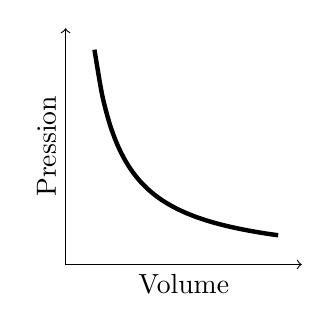
\begin{tikzpicture}[scale=\echelleGraphe]
  \node () at (\largeurGraphe*\facteurPositionTexteX,\hauteurGraphe*\facteurPositionTexteY) {$\reponseA$};
  \draw[<->] (0,\hauteurGraphe) -- (0,0) -- (\largeurGraphe,0);
  \draw[domain=(2-\facteurFinCourbe)*1/\hauteurGraphe:\largeurGraphe*\facteurFinCourbe,smooth,variable=\x,\blueOrBlack, ultra thick] plot ({\x},{1/\x});
  \node[below] at (\largeurGraphe*0.5,0) {Volume};
  \node[rotate=90,above] at (0,\hauteurGraphe*0.5) {Pression};
\end{tikzpicture}
%
\hfill
%
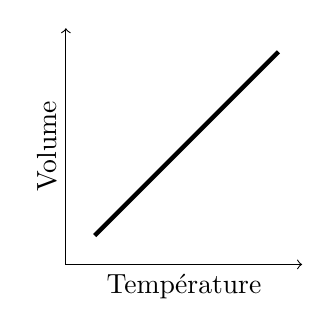
\begin{tikzpicture}[scale=\echelleGraphe]
  \node () at (\largeurGraphe*\facteurPositionTexteX,\hauteurGraphe*\facteurPositionTexteY) {$\reponseB$};
  \draw[<->] (0,\hauteurGraphe) -- (0,0) -- (\largeurGraphe,0);
  \draw[domain=(2-\facteurFinCourbe)*1/\hauteurGraphe:\largeurGraphe*\facteurFinCourbe,smooth,variable=\x,\blueOrBlack, ultra thick] plot ({\x},{\x});
  \node[below] at (\largeurGraphe*0.5,0) {Température};
  \node[rotate=90,above] at (0,\hauteurGraphe*0.5) {Volume};
\end{tikzpicture}
%
\hfill
%
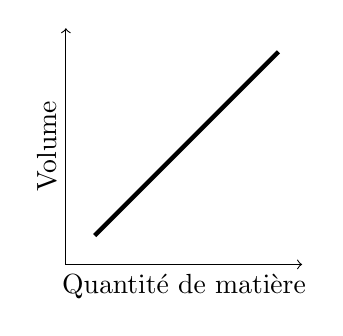
\begin{tikzpicture}[scale=\echelleGraphe]
  \node () at (\largeurGraphe*\facteurPositionTexteX,\hauteurGraphe*\facteurPositionTexteY) {$\reponseC$};
  \draw[<->] (0,\hauteurGraphe) -- (0,0) -- (\largeurGraphe,0);
  \draw[domain=(2-\facteurFinCourbe)*1/\hauteurGraphe:\largeurGraphe*\facteurFinCourbe,smooth,variable=\x,\blueOrBlack, ultra thick] plot ({\x},{\x});
  \node[below] at (\largeurGraphe*0.5,0) {Quantité de matière};
  \node[rotate=90,above] at (0,\hauteurGraphe*0.5) {Volume};
\end{tikzpicture}
%
\hfill
%
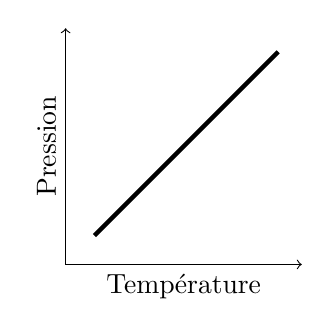
\begin{tikzpicture}[scale=\echelleGraphe]
  \node () at (\largeurGraphe*\facteurPositionTexteX,\hauteurGraphe*\facteurPositionTexteY) {$\reponseD$};
  \draw[<->] (0,\hauteurGraphe) -- (0,0) -- (\largeurGraphe,0);
  \draw[domain=(2-\facteurFinCourbe)*1/\hauteurGraphe:\largeurGraphe*\facteurFinCourbe,smooth,variable=\x,\blueOrBlack, ultra thick] plot ({\x},{\x});
  \node[below] at (\largeurGraphe*0.5,0) {Température};
  \node[rotate=90,above] at (0,\hauteurGraphe*0.5) {Pression};
\end{tikzpicture}
%
\hfill
%


